\chapter{Inflationary Cosmology}
\label{chap:cos}

\section{Introduction}
\label{sec:cos:intro}
I assume a working knowledge of Einstein's theory of general relativity. Review the key concepts mostly to establish notation. Excellent references can be found in~\cite{Wald},~\cite{Hobson} \&~\cite{Dodelson}.

\section{Einstein's gravity}
\label{sec:cos:einsteins_gravity}
\begin{quote}
  {\em Spacetime tells matter how to move;\\ matter tells spacetime how to curve.}\hfill
  --- \johnwheeler{}
\end{quote}

Einstein's theory of general relativity accounts for gravity by removing it as a fundamental ``force'' and replacing it as an effect of spacetime itself. Objects and fields still interact with one another on a spacetime background via the usual forces (electromagnetic, strong and weak nuclear forces). The spacetime itself can be thought of as being curved, and the effect of gravitation is due to objects moving on paths through a curved spacetime. Finally, the curvature is influenced by the matter content of the spacetime.

The formalism of Einstein's gravity can be effectively summarised using the Einstein-Hilbert action. An action $S$ is written as a general relativistic integral over a Lagrangian density $\mathcal{L}$:\footnote{This should not be confused with a likelihood, also denoted with $\lik$.}
\begin{equation}
  S = \int d^4 x \sqrt{|g|} \mathcal{L}.
  \label{eqn:cos:generic_lagrangian}
\end{equation}
where the factor of $\sqrt{g}$, $g=\left|\det\left( g_{\mu\nu} \right)\right|$ ensures a relativistic volume element for integration.
We typically decompose the Lagrangian $\mathcal{L}$ into a gravitational and matter part:
\begin{align}
  \mathcal{L} &= \mathcal{L}_G + \mathcal{L}_M
  \label{eqn:cos:decomp}\\
  \mathcal{L}_G &= \frac{1}{2} \m^2 R
  \label{eqn:cos:L_grav}
\end{align}
where $R$ is the Ricci scalar and $\mathcal{L}_M$ is the portion of the Lagrangian pertaining to the material content of spacetime. Requiring that the action~\eqref{eqn:cos:generic_lagrangian} is extremal ($\delta S = 0$) yields Einstein's equations:
\begin{equation}
 \m^2 G_{\mu\nu} = T_{\mu\nu},
  \label{eqn:cos:einsteins_equations}
\end{equation}
where
\begin{equation}
  T_{\mu\nu} = \frac{-2}{\sqrt{\abs{g}}}\frac{\delta}{\delta g^{\mu\nu}}\left( \sqrt{\abs{g} \mathcal{L}_M} \right)
  \label{eqn:cos:SET_fundamantal}
\end{equation}
is the stress energy tensor, and
\begin{equation}
  G_{\mu\nu} = R_{\mu\nu} - \frac{1}{2}g_{\mu\nu} R,
  \label{eqn:cos:einstein_tensor}
\end{equation}
is the Einstein tensor.

\section{The smooth, expanding universe}
\begin{table}
  \centering
\begin{tabular}{ll}
 \toprule
  Symbol & Definition \\
 \midrule
 \midrule
  $t$ & cosmic time \\
  $\chi$ & Comoving radial coordinate \\
  $\theta$ & polar angle \\
  $\phi$ & azimuthal angle \\
  $\Omega$ & solid angle \\
  $a$ & cosmic scale factor \\
  $k=+1$ & open universe \\
  $k=0$ & flat universe \\
  $k=-1$ & closed universe \\
 \bottomrule
\end{tabular}
\caption{Definitions of terms in the FRW metric}\label{tab:cos:metric}
\end{table}

On the largest scales, the universe is observed to be {\em homogeneous\/} and {\em isotropic}. This provides a good 0\textsuperscript{th}-order approximation to our actual universe. Making these assumptions, the metric can take one of three generic forms:
\begin{align}
  ds^2 &= dt^2 - a{(t)}^2\left( d\chi^2 + S_k^2{(\chi)} d\Omega \right)
  \label{eqn:cos:FRW_metric}\\
  d\Omega &= d\theta^2 + \sin^2\theta d\phi^2
  \label{eqn:cos:angle_element}\\
  S_k^2(\chi) &=
  \left\{
  \begin{array}{rl}
    \sin^2\chi &: k=+1 \\
    \chi^2 &: k=0 \\
    \sinh^2\chi &: k=-1. \\
  \end{array}
  \right.\label{eqn:cos:S_def}
\end{align}
The definitions of these terms can be found in Table~\ref{tab:cos:metric}. The scale factor $a(t)$ connects {\em comoving coordinates\/} $\chi$ with {\em physical coordinates}. Comoving variables can be thought of as a time-independent grid, which expand with the universe (Figure~\ref{fig:cos:comoving_vs_physical}). Physical coordinates are found by multiplying via the scale factor $a(t)$ to account for the effect of the expansion of the universe.
\begin{figure}
  \centering
  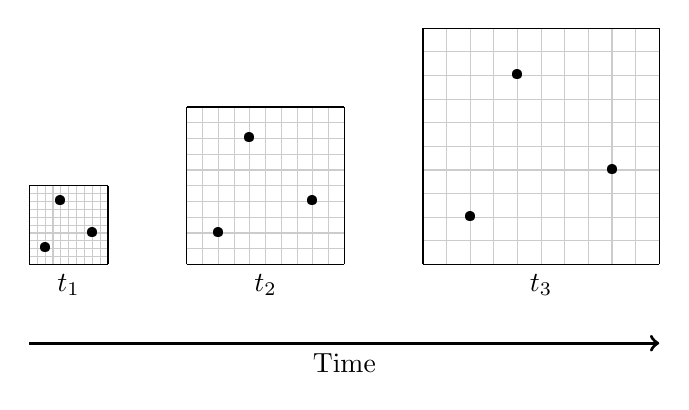
\begin{tikzpicture}
  % Draw the grids
  \draw[step=0.1,opacity=0.2] (0,0) grid (1,1);
  \draw[step=1] (0,0) grid (1,1);

  \draw[xshift=2cm,scale=2,step=0.1,opacity=0.2] (0,0) grid (1,1);
  \draw[xshift=2cm,scale=2,step=1] (0,0) grid (1,1);

  \draw[xshift=5cm,scale=3,step=0.1,opacity=0.2] (0,0) grid (1,1);
  \draw[xshift=5cm,scale=3,step=1] (0,0) grid (1,1);

  % Arrow of time
  \path[->, very thick] 
  (0,-1) 
  edge node[below] {Time}
  (8,-1);

  % Time Labels
  \node[below] at (0.5,0) {$t_1$};
  \node[below] at (3,0) {$t_2$};
  \node[below] at (6.5,0) {$t_3$};

  \def\xa{0.2} \def\ya{0.2}
  \def\xb{0.8} \def\yb{0.4}
  \def\xc{0.4} \def\yc{0.8}
  \def\object{\textbullet}

  \node[] (a1) at (\xa,\ya) {\object};
  \node[] (b1) at (\xb,\yb) {\object};
  \node[] (c1) at (\xc,\yc) {\object};

  \node[] (a2) at ({\xa*2 + 2},{\ya*2}) {\object};
  \node[] (b2) at ({\xb*2 + 2},{\yb*2}) {\object};
  \node[] (c2) at ({\xc*2 + 2},{\yc*2}) {\object};

  \node[] (a3) at ({\xa*3 + 5},{\ya*3}) {\object};
  \node[] (b3) at ({\xb*3 + 5},{\yb*3}) {\object};
  \node[] (c3) at ({\xc*3 + 5},{\yc*3}) {\object};


\end{tikzpicture}

  \caption{Comoving vs.\ physical coordinates.\label{fig:cos:comoving_vs_physical}}
\end{figure}




In order to obtain the equations governing $a(t)$ and thus the dynamics of the universe, we must make some assumptions about the universes contents. For a smooth universe, one may model its contents as a collection of non-interacting, comoving, uniform, perfect fluids. A perfect fluid in thermodynamic equilibrium has stress-energy tensor:
\begin{equation}
  T^{\mu\nu} = (P+\rho)u^{\mu}u^{\nu} - P g^{\mu\nu} + \Sigma^{\mu\nu}
  \label{eqn:cos:SET_perfect_fluid}
\end{equation}
where $\rho$ is the energy density, $P$ is the pressure, $u^\mu$ is the four velocity of the fluid, and $\Sigma^{\mu\nu}$ is a traceless, symmetric, anisotropic stress term. In accordance with the cosmological principle, we shall assume that in the comoving frame the fluid is stationary ($u^\mu = [1,\bzero]$), and uniform ($\rho=\rho(t),P=P(t)$), with no anisotropy $\Sigma=0$.  

Applying the metric~\eqref{eqn:cos:FRW_metric} to the Einstein equations~\eqref{eqn:cos:einsteins_equations}, with the stress-energy tensor~\eqref{eqn:cos:SET_perfect_fluid} one finds:
\begin{align}
  \dot{H}+H^2 &= 
  -\frac{1}{6\m^2}\left( \rho + 3P\right), 
  \label{eqn:Raychaudhuri_rho}
  \\
  H^2 &= 
  \frac{1}{3\m^2}\rho - \frac{k}{a^2}, 
\end{align}
%
where $H=\dot{a}/a$ is the Hubble parameter and a dot denotes differentiation with respect to cosmic time, $\dot{f}\equiv df/dt$. These are termed the {\em Raychaudhuri\/} and {\em Friedmann\/} equations respectively, and implicitly govern the dynamics of the scale factor $a(t)$. 


 Typically we will assume that the universe is flat $(k=0)$ for simplicity, although most analyses can be extended to the open or closed cases. In the flat case, we may write the spatial part with vectors:
\begin{equation}
  ds^2 = dt^2 - a{(t)}^2 d{\vx}^2.
  \label{eqn:cos:flat_FRW}
\end{equation}
It is also convenient to define conformal time as:
\begin{equation}
  \eta = \int \frac{dt}{a},
  \label{eqn:cos:conformal_time}
\end{equation}
so that the line element becomes:
\begin{equation}
  ds^2 = a(\eta)\left( dt^2 - d{\vx}^2 \right).
  \label{eqn:cos:flat_FRW}
\end{equation}
Here, one can see that the metric is now conformally equivalent to Minkowski space\footnote{hence the name ``conformal time''.}.
This is often analytically useful, but physically conformal time corresponds to a time coordinate in which photons travel in straight lines. Alternatively, it is the time measured by a small light clock that expands comovingly with the universe. It can also be thought of as a ``comoving'' time. Most usefully, if the lower end of the integral in~\eqref{eqn:cos:conformal_time} is the origin of the universe, then this amounts to the largest comoving distance that light could have travelled by that moment in time.
                                                                     
\section{Cosmic Horizons}
There are several useful scales in cosmology. The first is the Hubble radius and Hubble time:
\begin{equation}
  \text{Hubble time} = \frac{1}{H} = \text{Hubble radius}.
  \label{eqn:cos:Hubble_def}
\end{equation}
The Hubble time is the timescale on which the universe approximately doubles in size. Since the speed of light $c=1$, this is also equal to the Hubble radius, which is approximately the distance over which particles can communicate subluminally over a Hubble time.

The second scale is the comoving Hubble radius:
\begin{equation}
  \text{conformal Hubble time} = \frac{1}{aH} = \text{comoving Hubble radius}.
  \label{eqn:cos:com_Hubble_def}
\end{equation}
This is very similar to the physical Hubble radius and time, but now represented in comoving coordinates.

%\section{The $\Lambda$CDM concordance cosmology}
%
%\begin{figure}
%\centering
%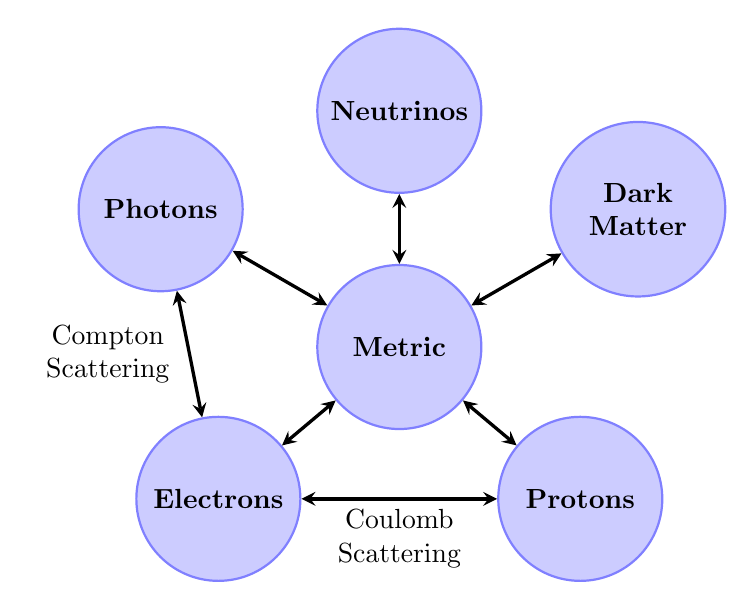
\begin{tikzpicture}[%
    writing/.style={%
      text width=18mm,  % default text width
      align=center      % align in center
    },
    component/.style={%
      circle,           % circular node
      fill=blue!20,     % fill it in blue
      draw=blue!50,     % outside edge in blue
      thick,            %              and thick
      writing,          % writing style above
      font=\bfseries    % bold writing
    },
    connection/.style={%
      <->,             % Double headed
      very thick,      % very thick arrows
      >=stealth        % pretty arrow head
    }
]

    % nodes
    \node at (0,0)     [component] (metric)      {Metric};

    \node at (90 :3)   [component] (neutrinos)   {Neutrinos};
    \node at (150:3.5) [component] (photons)     {Photons};
    \node at (220:3)   [component] (electrons)   {Electrons};    
    \node at (320:3)   [component] (protons)     {Protons};      
    \node at (30 :3.5) [component] (dark matter) {Dark Matter};


    % connections
    \draw[connection] (metric) -- (neutrinos);
    \draw[connection] (metric) -- (photons);
    \draw[connection] (metric) -- (electrons);
    \draw[connection] (metric) -- (protons);
    \draw[connection] (metric) -- (dark matter);

    % interconnections with text
    \draw[connection] 
    (electrons) to 
    node[below,writing] {Coulomb Scattering} 
    (protons);

    \draw[connection] 
    (electrons) to 
    node[left,writing] {Compton Scattering} 
    (photons);

\end{tikzpicture}

%\caption{Composition of the universe, along with the interaction of the components.\label{fig:cos:composition}}
%\end{figure}


\section{Inflation}
The canonical way to explain this early accelerated phase is via the phnomenon of {\em inflation}.


\clearpage{}

